\section{Experiments}
\label{sec:exp}

\paragraph{Common setup.} All experiments use Qwen2.5-Coder-7B-Instruct with LoRA
($r{=}16$), greedy decoding, batch size 10, window $W{=}9$, $k$NN $k{=}3$
(Qwen3-Embedding-0.6B), seed-42 stream order identical across methods. Baselines:
\textbf{Base} (zero-shot, no adaptation), \textbf{ICL} (Self-StreamICL: reward-filtered
memory + $k$NN demos, frozen weights), and \textbf{REINFORCE++} (policy gradient with
global-whitened advantages, PPO clipping, KL to the frozen base, replaying stored
completions over the same rolling window). All methods see identical problems in
identical order; base, ICL, and REINFORCE++ use exactly one oracle call per problem
(cost accounting for SDFT in \S\ref{sec:exp-ablations}).

\subsection{Seven streaming benchmarks}
\label{sec:exp-bench}

Table~\ref{tab:bench} reports each benchmark's native accuracy over its full
stream. \textbf{Our method attains the best accuracy on all seven tasks}, spanning
competitive code generation, data-science code, two text-to-SQL tasks, medical
diagnosis, multi-hop QA, and function calling. Two patterns recur. First, ICL is a
strong baseline where retrieval finds near-duplicates (DDXPlus) but can
\emph{hurt} on tasks where retrieved demonstrations mislead (HotpotQA: $0.509$ vs
base $0.521$); self-distillation recovers and surpasses base in exactly those
cases ($0.562$), because the signal is consolidated in weights rather than
recalled at inference. Second, REINFORCE++ is inconsistent---above ICL on some
tasks, far below base on others (Spider $0.587$ vs $0.747$)---previewing the
stability failure of \S\ref{sec:exp-fused}.

\begin{table}[t]
\centering
\caption{Streaming accuracy on seven StreamBench tasks (native metric per task;
identical stream order and model for all methods). Our method is best on all
seven.}
\label{tab:bench}
\begin{tabular}{llrrrrr}
\toprule
Benchmark & Domain & Size & Base & ICL & R++ & \textbf{Ours} \\
\midrule
LiveCodeBench & code & 1055 & 0.338 & 0.424 & 0.386 & \textbf{0.448} \\
DS-1000 & Python & 955 & 0.325 & 0.367 & 0.369 & \textbf{0.423} \\
Spider & text-to-SQL & 2147 & 0.747 & 0.778 & 0.587 & \textbf{0.808} \\
DDXPlus & medical dx & 1764 & 0.436 & 0.647 & 0.404 & \textbf{0.664} \\
BIRD & hard SQL & 1534 & 0.330 & 0.346 & 0.271 & \textbf{0.354} \\
HotpotQA & multi-hop QA & 1500 & 0.521 & 0.509 & 0.537 & \textbf{0.562} \\
ToolBench & func-calling & 750 & 0.549 & 0.593 & 0.607 & \textbf{0.615} \\
\bottomrule
\end{tabular}

\end{table}

\subsection{Distribution shift: one model, three domains}
\label{sec:exp-fused}

We interleave DS-1000 (code, 955), DDXPlus (diagnosis, 1{,}764), and HotpotQA
(QA, 1{,}500) into a single 4{,}219-problem stream by a random merge that
\emph{preserves each domain's internal order}, making per-domain slices exactly
comparable to the standalone runs. Table~\ref{tab:fused} shows the outcome.

\begin{table}[t]
\centering
\caption{Fused-stream results (4{,}219 problems). ``SDFT standalone'' aggregates
the three per-domain runs at matched prefixes (regret summed, accuracy weighted).
One online-distilled model matches or beats three specialists.}
\label{tab:fused}
\begin{tabular}{lrrrrr}
\toprule
Method & Acc & Cum.\ regret & DS-1000 & DDXPlus & HotpotQA \\
\midrule
Base & 0.439 & 2365 & 0.318 & 0.436 & 0.521 \\
ICL $k{=}3$ & 0.533 & 1971 & 0.358 & 0.647 & 0.509 \\
REINFORCE++ (fused) & 0.253 & 3153 & 0.213 & 0.262 & 0.267 \\
SDFT standalone ($3\times$) & 0.573 & 1800 & 0.423 & 0.664 & \textbf{0.562} \\
\textbf{SDFT fused (ours)} & \textbf{0.585} & \textbf{1750} & \textbf{0.457} & \textbf{0.676} & 0.560 \\
\bottomrule
\end{tabular}

\end{table}

Three findings. \textbf{(i) One model $\geq$ three specialists:} the fused model
beats the aggregated standalone runs overall ($.585$ vs $.573$) and is no worse on
any domain, with \emph{positive} cross-domain transfer to code ($+3.4$ points on
DS-1000). \textbf{(ii) Transfer lives in the weights:} retrieval self-segregates
---99.9\% of retrieved demonstrations are same-domain (2 of 2{,}059 queries pull
any cross-domain demo)---so prompts are effectively domain-pure and cannot explain
the gains. \textbf{(iii) RL collapses:} REINFORCE++ tracks ${\sim}5$ points below
SDFT for 2{,}000 problems, then diverges catastrophically (approximate KL turns
negative, clip fraction spikes $0.08{\to}0.68$, advantage std triples); accuracy
falls to zero for the remainder of the stream (final $0.253$). The same
hyperparameters are stable on every shorter standalone stream, indicating a
long-horizon instability that online self-distillation simply does not exhibit:
its per-window KL objective is anchored to a frozen teacher and its rolling
accuracy climbs monotonically ($.44 \to .68$ peak) over the same stream
(Figure~\ref{fig:trend}).

\begin{figure}[t]
\centering
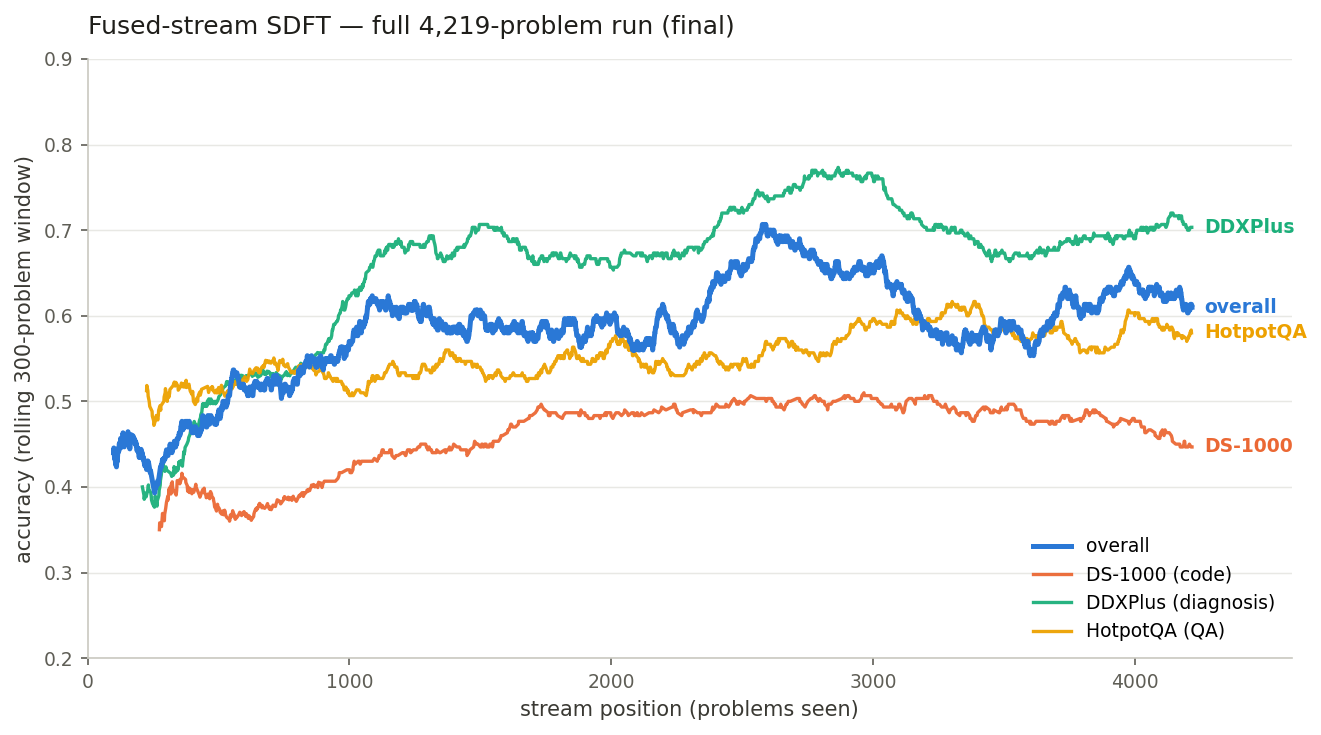
\includegraphics[width=0.9\linewidth]{figures/fused_accuracy_trend.png}
\caption{Rolling accuracy (300-problem window) of online SDFT over the fused
three-domain stream, overall and per domain. All domains improve simultaneously;
no interference from distribution shift.}
\label{fig:trend}
\end{figure}

\subsection{Online vs.\ batch training}
\label{sec:exp-transfer}

Does the \emph{online schedule itself} matter, beyond the loss? We compare our
online run on DS-1000 against \emph{batch} self-distillation: the identical
trainer, loss, model, and oracle, but run as classic offline epochs (4 passes over
all 955 problems; per pass: generate, oracle-filter, distill on verified answers;
no memory, no stream). We then evaluate both resulting adapters with a single
bare-prompt greedy pass over the full problem set (no demonstrations, no memory).

\begin{table}[h]
\centering
\caption{Source-data mastery after training on DS-1000 (bare-prompt greedy pass,
all 955 problems).}
\label{tab:mastery}
\begin{tabular}{lrr}
\toprule
Model & Acc & Solved / 955 \\
\midrule
Base & 0.313 & 313 \\
Batch SDFT (4 epochs) & 0.425 & 406 \\
\textbf{Online SDFT (ours)} & \textbf{0.480} & \textbf{458} \\
\bottomrule
\end{tabular}

\end{table}

The online-trained model solves $458/955$ ($.480$) versus $406$ ($.425$) for
batch---a $+5.5$-point gap \emph{on the very data batch trained on for four
epochs}---and its advantage comes from breadth: 123 problems only online solves vs
71 only batch solves, with equal (small) forgetting relative to base. We attribute
the gap to the stream's implicit curriculum: each problem is revisited across a
rolling window while the model evolves, and forward re-evaluation keeps
converting newly in-reach problems into training signal, whereas single-sample
batch generation can only ever train on what the current model already solves.
\todo{Batch with $n{=}5$ sampled attempts per problem (running) tests whether
exploration closes this gap.}
\todo{Transfer: both adapters warm-start online SDFT on the unseen HotpotQA
stream; compare accuracy/regret vs from-scratch ($.562$/657). Runs pending.}

\subsection{Ablations and cost}
\label{sec:exp-ablations}

\textbf{Generation source.} Sampling the distillation completion from the bare
student prompt (offline-SDFT default) vs the hint-conditioned prefix (ours)
changes DS-1000 by $+1.3$ points in favor of the former, with the difference
confined to the early stream; on the fused stream the two are even after a small
early deficit. The choice is a bootstrap-phase detail, not a driver.
\textbf{Epochs.} 4 inner epochs beat 2 on DS-1000 ($+21$ cumulative-regret at
matched pressure); learning-rate increases do not substitute for epochs.
\textbf{Multi-sample distillation.} Distilling from $N{=}10$ sampled candidates
(filtered or not) matches single-sample distillation---sample \emph{count} is not
the bottleneck.
\textbf{Oracle budget.} Our method issues ${\sim}9.8$ oracle calls per problem
(1 scored on arrival + ${\sim}8.8$ memory-only re-evaluations); baselines use 1.
The extra calls only gate memory; they never alter recorded scores. Giving ICL
the same budget would not help---a frozen model re-answering with the same
distribution recovers almost nothing---and REINFORCE++ at 1 call/problem already
shows that training-with-feedback alone does not close the gap.
